\chapter{Working Example}

To demonstrate the major stages and purpose of the simulator we shall make extensive use of the examples in this chapter.
For simplicity we have chosen to use Bitonic Sorting.

\section{Bitonic Sorting Overview}

\begin{figure}
\begin{center}
	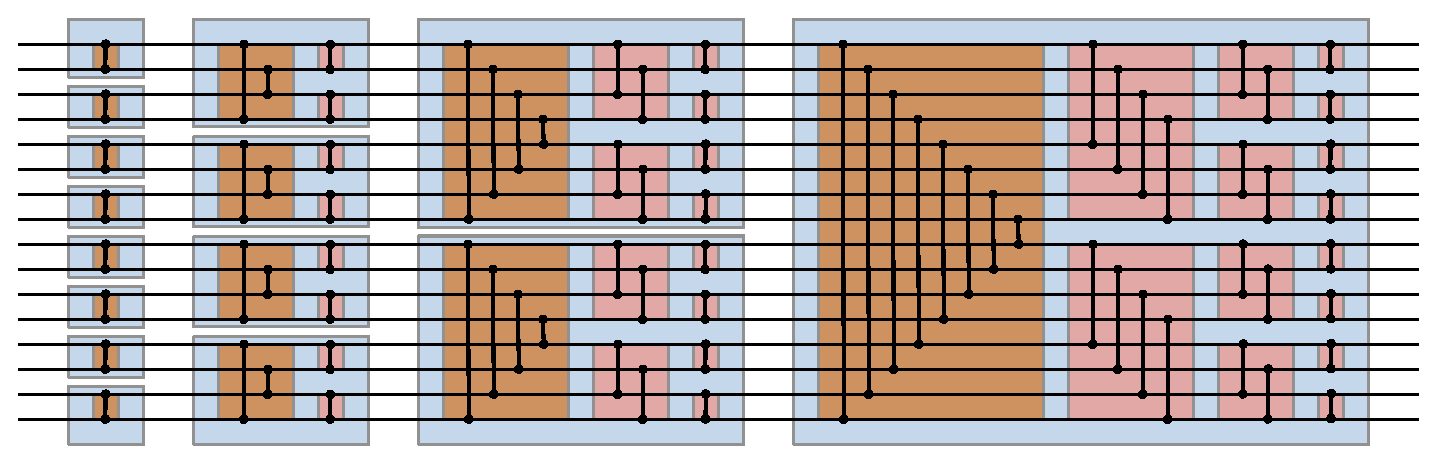
\includegraphics[width=12cm]{figures/egBitonicSort.eps}
\caption{The major stages of bitonic sort.  Image from Wikipedia: Bitonic Sorter}
\label{figBitonicNormal}
\end{center}
\end{figure}

Bitonic sorting is a common distributed sorting network.
Sorting is a well known and studied task, so it makes sense to use this as our working example.
We choose this method over more well known algorithms (merge, quick, bubble, selection) because it has interesting distributed properties.
In its basic form, a sequence is bitonic if it can be expressed in the form $x_0 \leq x_1 \leq ... \leq x_k \geq x_{k+1} \geq ... \geq x_{n-1}$ for $n$ elements and some $k$.

Figure \ref{figBitonicNormal} shows a bitonic sorting network for sixteen items.
This is a variation on the more well known bitonic sorting networks which allows us to ignore the up/down sorting complexity.
In this diagram items cross from left to right in line.
When two items reach a crossbar they swap location if the lower one has a lesser value than the higher, otherwise they do not swap.
This figure also shows the major stages of the sorting process.
Each box (orange, pink and blue) is isolated from crossovers in the same box, in other words, they may be scheduled in parallel.
At the right edge of each blue box, all the channels are sorted, this demonstrates the divide-and-conquer nature of the network, each box can therefore be though of as distributed merging steps.

Bitonic sort was one of the first distributed parallel sorting algorithms known to take $O(\log^2 n)$ time.
However this bound requires some reasonable and some arguably naive assumptions.
The time bound arises from the observations that each stage can sort twice as many elements as the last, for one more internal block.
Hence at most $\log n$ stages with the largest one having at most $\log n$ blocks are required.
But this assumes that communication can be dome in unit time, which in practice is not true due to overheads.
More specifically for our analysis communication overheads are larger when forming connections, so this sorting network will suffer somewhat from the proposed checkpoint-recovery scheme.
Further, this time complexity requires $O(n)$ to work in parallel (more accurately, $n/2$).
Indeed the total time complexity (on a single machine) is $O(n \log^2 n)$, in other words $\log n$ times worse than merge sort.
So in order to sort 64 items quickly, a full 32 machines are required.
This problem may be exacerbated by the requirement to also duplicate each actor for the replication fault-tolerance scheme.

\section{SDF Graph}

\begin{figure}
\begin{center}
	\begin{pspicture}(10,6)
	
	\cnode(3,4.2){0.4}{a}
	\cnode(3,1.8){0.4}{b}
	\cnode(5,4.2){0.4}{c}
	\cnode(5,1.8){0.4}{d}
	\cnode(7,4.2){0.4}{e}
	\cnode(7,1.8){0.4}{f}
	
	\cnodeput(1,3){i}{Input}
	\cnodeput(9,3){o}{Output}
	
	\nccurve[angleA=60,angleB=180]{->}{i}{a}
	\nccurve[angleA=20,angleB=180]{->}{i}{a}
	\nccurve[angleA=-20,angleB=180]{->}{i}{b}
	\nccurve[angleA=-60,angleB=180]{->}{i}{b}
	
	\nccurve[angleA=20,angleB=180]{->}{a}{c}
	\nccurve[angleA=-20,angleB=180]{->}{a}{d}
	\nccurve[angleA=20,angleB=180]{->}{b}{d}
	\nccurve[angleA=-20,angleB=180]{->}{b}{c}
	
	\nccurve[angleA=20,angleB=180]{->}{c}{e}
	\nccurve[angleA=-20,angleB=180]{->}{c}{f}
	\nccurve[angleA=20,angleB=180]{->}{d}{e}
	\nccurve[angleA=-20,angleB=180]{->}{d}{f}
	
	\nccurve[angleA=20,angleB=120]{->}{e}{o}
	\nccurve[angleA=-20,angleB=160]{->}{e}{o}
	\nccurve[angleA=20,angleB=200]{->}{f}{o}
	\nccurve[angleA=-20,angleB=240]{->}{f}{o}

\end{pspicture}
\caption{The bitonic sort in SDF form.}
\label{figBitonicGraph}
\end{center}
\end{figure}

Figure \ref{figBitonicGraph} shows the bitonic sort for four elements as a SDF graph.
For clarity the channel cardinalities are omitted, since they all have 1 production and 1 consumption per invocation.
It should be said that this graph depicts the sort for four items, however in actual tests with the simulator (see Chapter \ref{chapSystems}) the sorting network is dynamically generated to sort $2^n$ items, for some n.

The function of each actor (except the input and output nodes) is the same.
The actor receives inputs in some order, and emits the lesser token on its upper channel, and the other on its lower channel.
Unfortunately the horizontal channels in Figure \ref{figBitonicNormal} become distorted in this depiction, however in function this graph is identical to the first two blue box stages for the upper four channels in that figure.
Since it doesn't matter which of the input tokens is greater (only the output ones) the diagram joins the arcs where they enter the nodes, however this is simply for clarity and doesn't affect the computation.

The input and output nodes have basic functionality.
For convenience's sake we can think of the input node as generating random numbers for each of its channels, and the output node as printing the numbers from top to bottom.
In the actual implementation, the output node checks the correctness of the ordering, which may be wrong under certain faults.
In a real-world use this graph would be a component of a larger system, and so it may not even have designated input and output nodes.

\section{Issues}

It may be useful at this point to analyse and consider the possible implications of the working example we have chosen.
In this way we will be able to compare intuitive notions of the problem with actual results.

Actors in this network are extremely light weight.
Many SDF implementations, including StreamIt, are designed to allow user-coded actors, and these actors can in practice become quite heavy.
In contrast the actors in our example do a comparison and then output the tokens immediately.
This may hide complexities in fault-tolerance, however for now it is sufficient to treat the actors as black boxes regarding fault tolerance.

Similarly, the channels in this network are well ordered, uniform and have no delays.
Well ordered channels can be given definite precedence, i.e. we can say that tokens passing through parts ``later'' in the graph had to go through ``earlier'' channels.
This ordering inherently means that there are no cycles, as this would require certain channels to precede themselves.
In the case of bitonic sort, the ordering is very apparent (left to right as per Figure \ref{figBitonicGraph}), and allows us to saturate the network with delays easily with little buffering requirements.
Certain SDF graphs are much harder to saturate than this example, however since scheduling and initialising are not focus areas for this work we can safely marginalise this issue.

The uniformity in the channels is also unrepresentative of SDF graphs in general.
In our case this causes the repetitions to be one for all actors per steady state invocation.
This may allow for some simplifications regarding the checkpointing mechanism, however it does not seem that it will make either method more or less clearly effective.

Delays are an important feature of SDF programs, especially where cycles are involved.
In the case where our graph has no delays this simplifies the partitioning and assignment problems, however we presume it does not noticeably affect the faultiness in the system.

\section{Other examples}

Though these examples will not feature prominently in the remainder of this work, it may be helpful to consider them.

\subsection{High Cardinality Repetitions}

\begin{figure}
\begin{center}
	\begin{pspicture}(10,4)
	
	\cnode(1.5, 2){0.7}{a}
	\cnode(5, 2){0.7}{b}
	\cnode(8.5, 2){0.7}{c}
	
	
	\ncline{->}{a}{b}
	\aput(0.15){3}
	\aput(0.85){7}
	\ncline{->}{b}{c}
	\aput(0.15){2}
	\aput(0.85){5}

\end{pspicture}

\caption{A SDF graph with deceptively high cardinality.}
\label{figCardinality}
\end{center}
\end{figure}

Figure \ref{figCardinality} shows an artificial SDF graph with an important property.
If we calculate the repetitions vector of this graph, as shown in \ref{figCardinalityMaths} we see that the number of times each actor is invoked far exceeds the number needed to fulfil the invocation of any one actor.
Indeed the buffer for the left-most channel may require storage for up to 105 tokens if the left actor executes all thirty five times before the middle actor executes at all.

We have contrived this example by chaining channels with prime consumption and production amounts together.
However this explosion in repetitions can be brought about simply by having monotonically increasing channels.
For example if each actor requires two tokens from its left neighbour and provides one to its right, then a chain of eight actors will require the left most to execute 256 times.

Graphs of this kind are not of much direct interest to our work.
Admittedly larger invocation vectors cause difficulties in checkpointing due to sheer volume of data, it may be interesting to gauge by how much.
However graphs with this property are of interest to performance-seeking optimisations, which may indirectly affect fault tolerance.

One strategy for dealing with huge invocation amounts is to {\em fiss} the actors.
Fissing is described by Thies et al and Malke in \cite{thies02, mal08} as splitting stateless actors into multiple versions of themselves.
This technique would inevitably cause overheads for fault tolerance, checkpointing of fissed actors may require extra detail to account for the split, and since these actors are split for performance reasons, duplicating their computations may be unappealing.

\begin{figure}
\begin{center}
\[
 \Gamma = \begin{bmatrix}
	3 & -7 & 0 \\
	0 & 2 & -5 \\
     \end{bmatrix}
	q = \begin{bmatrix}
	35 \\
	15 \\
	6 \\
     \end{bmatrix}
\]
\caption{The topology matrix and repetitions vector for the graph in Figure \ref{figCardinality}}
\label{figCardinalityMaths}
\end{center}
\end{figure}

\subsection{Feedback}

\begin{figure}
\begin{center}
	\begin{pspicture}(10,6)
	
	\cnodeput(1.5,2.5){a}{Add}
	\cnodeput(5,2){d1}{Dup}
	\cnodeput(5,4){d2}{Dup}
	\cnodeput(8.5,3.5){o}{Output}
	
	\nccurve[angleA=270,angleB=270]{->}{a}{d1}	\aput(0.15){1} \aput(0.85){1}
	\nccurve[angleA=180,angleB=0]{->}{d1}{a}	\bput(0.15){1} \bput(0.85){1}
	\bput(0.5){$[0]$}
	\nccurve[angleA=90,angleB=270]{->}{d1}{d2}	\aput(0.15){1} \aput(0.85){1}
	\nccurve[angleA=180,angleB=90]{->}{d2}{a}	\bput(0.15){1} \bput(0.85){1}
	\bput(0.5){$[1, 0]$}
	\nccurve[angleA=0,angleB=180]{->}{d2}{o}	\aput(0.15){1} \aput(0.85){1}

\end{pspicture}

\caption{A SDF graph to compute the Fibonacci sequence.}
\label{figFibonacci}
\end{center}
\end{figure}

Figure \ref{figFibonacci} shows a SDF graph which emits the Fibonacci sequence to the output node.
The functions of the actors is fairly self explanatory, however we can see cycles (add-dup, add-dup-dup) and delays (in square brackets) in this graph.
These features are once again important for performance analysis reasons, however we can largely ignore them.

The main difficulty that feedback introduces is that saturating the network becomes difficult.
One strategy is to treat the SDF graph as a directed graph aggregate the strongly connected components using Tarjan's algorithm to obtain a directed acyclic graph, however that is outside the scope of this thesis.
Cycles in the graph do not directly increase the communication requirements or dependencies, so out fault-tolerance mechanisms are unaffected by this property where it exists.